\documentclass{beamer}

\usepackage[brazil]{babel}
\usepackage[utf8]{inputenc}
\usepackage[T1]{fontenc}

\usetheme{Madrid}
\setbeamertemplate{navigation symbols}{}

\title[Lógica Computacional]{Lógica Computacional}

\author[Diego S. C. Nascimento]{Diego Silveira Costa Nascimento}

\institute[IFRN]{
Instituto Federal de Educação, Ciência e Tecnologia do Rio Grande do Norte\\
diego.nascimento@ifrn.edu.br
}

\date[\today]{\today}

\begin{document}

\begin{frame}[plain]
	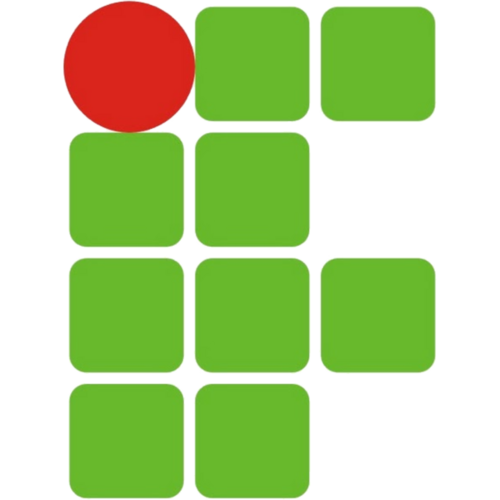
\includegraphics[scale=0.2]{img/IFRN}
	\titlepage
\end{frame}

\logo{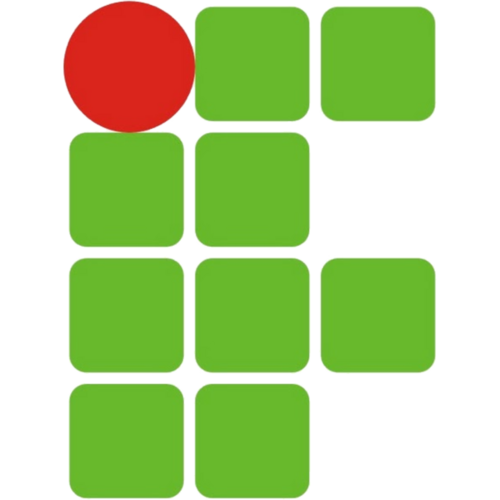
\includegraphics[scale=0.1]{img/IFRN}}

\begin{frame}
	\frametitle{Ementa do Curso}
  	\tableofcontents
\end{frame}

\AtBeginSection[]{
	\begin{frame}
		\frametitle{Ementa do Curso}
		\tableofcontents[currentsection]
	\end{frame}
}

\section{Introdução}

\begin{frame}
	\frametitle{Lógica}

	\begin{block}{Definição}
		É a ciência das leis ideais do pensamento e a arte de aplicá-las à pesquisa e à demonstração da verdade.
	\end{block}\vfill
	
	\begin{itemize}
		\item Deriva do Grego (logos); e
		\item Significa:
			\begin{itemize}
			\item palavra;
			\item pensamento;
			\item ideia;
			\item argumento;
			\item relato;
			\item razão
			\item lógica; ou
			\item princípio lógico.
			\end{itemize}
	\end{itemize}
\end{frame}

\begin{frame}
\frametitle{Origem}

\begin{itemize}
	\item A Lógica teve início na Grécia em 342 a.C.;
	\item Aristóteles sistematizou os conhecimentos existentes em Lógica, elevando-a à categoria de ciência;
	\item Obra chamada Organon (Ferramenta para o correto pensar);
	\item Aristóteles preocupava-se com as formas de raciocínio que, a partir de conhecimentos considerados verdadeiros, permitiam obter novos conhecimentos; e
	\item A partir dos conhecimentos tidos como verdadeiros, caberia à Lógica a formulação de leis gerais de encadeamentos lógicos que levariam à descoberta de novas verdades.
\end{itemize}\vfill

\begin{columns}[c] 
	\column{.3\textwidth}
	\begin{exampleblock}{Aristóteles}
		\center
		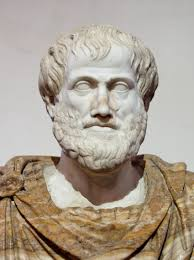
\includegraphics[scale=0.18]{img/aristoteles}
	\end{exampleblock}
	
	\column{.3\textwidth}
	\begin{exampleblock}{Organon}
		\center
		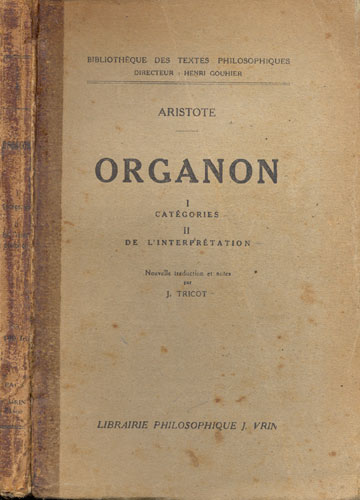
\includegraphics[scale=0.1]{img/organon}	
	\end{exampleblock}
	
\end{columns}
\end{frame}

\begin{frame}
\frametitle{Princípios Lógico}

A Lógica Formal repousa sobre três princípios fundamentais que permitem todo seu desenvolvimento posterior, e que dão validade a todos os atos do
pensamento e do raciocínio.

\begin{exampleblock}{Princípio da Identidade}
Afirma $A = A$ e não pode ser $B$, o que é, é.
\end{exampleblock}\vfill
	
\begin{exampleblock}{Princípio da Não Contradição}
$A = A$ e nunca pode ser não-$A$, o que é, é e não pode ser sua negação, ou seja, o ser é, o não ser não é.
\end{exampleblock}\vfill

\begin{exampleblock}{Princípio do Terceiro Excluído}
Afirma que Ou $A$ é $x$ ou $A$ é $y$, não existe uma terceira possibilidade.
\end{exampleblock}

\end{frame}

\section{Lógica Proposicional}

\begin{frame}
\frametitle{Proposição}

\begin{itemize}
	\item Chama-se proposição todo o conjunto de palavras ou símbolos que exprimem um pensamento de sentido completo;
	\item As proposições transmitem pensamentos; e
	\item Afirmam fatos ou exprimem juízos que formamos a respeito de determinados entes.
\end{itemize}\vfill

\begin{exampleblock}{Exemplos}
A Lua é um satélite da terra\\
Sócrates é um homem\\
Eu estudo lógica\\
Não está chovendo
\end{exampleblock}
\end{frame}

\begin{frame}
\frametitle{A Linguagem}

\begin{block}{Considere o conjunto de símbolos:}
$ A = \{(,), \neg, \wedge, \vee, \rightarrow, \leftrightarrow, p, q, r, ... \}$
\end{block}\vfill

\begin{itemize}
	\item A esse conjunto é chamado de alfabeto da Lógica Proposicional;
	\item As letras são símbolos não lógico (letras sentenciais); e
	\item O restante são símbolos lógicos (parênteses e conectivos lógicos).
\end{itemize}
\end{frame}

\begin{frame}
\frametitle{Letras Sentenciais}

As letras sentenciais são usadas para representar proposições elementares ou atômicas, isto é, proposições que não possuem partes que sejam também proposições.
\vfill
\begin{exampleblock}{Exemplos}
p = O céu é azul\\
Q = Eu estudo lógica\\
r = 2 + 2 = 4\\
s = Sócrates é um homem
\end{exampleblock} \vfill

\begin{alertblock}{Importante}
As partes dessas proposições não são proposições mais simples, mas sim, componentes subsentenciais: expressões, palavras, sílabas ou letras.
\end{alertblock}
\end{frame}

\begin{frame}
\frametitle{Conectivos Lógicos}

\begin{itemize}
	\item As proposições compostas são obtidas combinando proposições simples através de certos termos chamados conectivos;
	\item A Lógica dispõe de cinco tipos de conectivos e seus operadores:
	\begin{itemize}
		\item Não (Negação), \structure{$\neg$};
		\item E (Conjunção), \structure{$\wedge$};
		\item Ou (Disjunção), \structure{$\vee$};
		\item Se -- então (Condicional), \structure{$\rightarrow$};e
		\item Se e somente se (Bicondicional), \structure{$\leftrightarrow$}.
	\end{itemize}
\end{itemize}
\end{frame}

\begin{frame}
\frametitle{Operador de Negação}

A característica peculiar da negação, tal como ela se apresenta na lógica proposicional clássica, é que toda proposição submetida à operação de negação resulta na sua contraditória. \vfill

\begin{exampleblock}{Exemplos}
$p =$ Está chovendo.\\
Ler-se $\neg p$, como: ``\structure{Não} está chovendo''.
\end{exampleblock}
\end{frame}

\begin{frame}
\frametitle{Tabela-verdade para Negação}

\begin{itemize}
	\item Se $p$ é uma proposição, a expressão $\neg p$ é chamada negação de $p$; e
	\item Claramente, a negação inverte o valor verdade de uma expressão.
\end{itemize} \vfill

\begin{exampleblock}{Exemplos}
\center
\begin{tabular}{|c|c|}
\hline
\textbf{p} & \textbf{$\neg$p}\\ \hline
V & F \\ \hline
F & V \\ \hline
\end{tabular}
\end{exampleblock}
\end{frame}

\begin{frame}
\frametitle{Operador de Conjunção}

A característica peculiar da conjunção está no fato de fórmulas conjuntivas expressarem a concomitância de fatos. A fórmula $(p \wedge q)$ expressa que o
fato expresso por $p$ ocorre ao mesmo tempo que o fato expresso por $q$. \vfill

\begin{exampleblock}{Exemplos}
$p =$ Está chovendo.\\
$q =$ Está ventando.\\
Ler-se $p \wedge q$, como: ``Está chovendo \structure{e} está ventando.''
\end{exampleblock}
\end{frame}

\begin{frame}
\frametitle{Tabela-verdade para Conjunção}

\begin{itemize}
\item Se $p$ e $q$ são proposições, a expressão $p \wedge q$ é chamada conjunção de $p$ e $q$; e
\item As proposições $p$ e $q$ são chamadas fatores da expressão.
\end{itemize} \vfill

\begin{exampleblock}{Exemplos}
\center
\begin{tabular}{|c|c|c|}
	\hline
	\textbf{p} & \textbf{q} & \textbf{p $\wedge$ q}\\ \hline
	V & V & V \\ \hline
	V & F & F \\ \hline
	F & V & F \\ \hline
	F & F & F \\ \hline
\end{tabular}
\end{exampleblock}
\end{frame}

\begin{frame}
\frametitle{Operador de Disjunção}

A característica peculiar da disjunção consiste no fato de proposições disjuntivas expressarem que pelo menos um de dois fatos ocorre. A fórmula $(p \vee q)$ expressa que, dentre os fatos expressos por $p$ e $q$ respectivamente,
pelo menos um deles ocorre. \vfill

\begin{exampleblock}{Exemplos}
$p =$ Está nublado.\\
$q =$ Está chovendo.\\
Ler-se $p \vee q$, como: ``Está nublado \structure{ou} está chovendo.''
\end{exampleblock}
\end{frame}

\begin{frame}
\frametitle{Tabela-verdade para Disjunção}

\begin{itemize}
\item Se $p$ e $q$ são proposições, a expressão $p \vee q$ é chamada disjunção inclusiva de $p$ e $q$; e
\item As proposições $p$ e $q$ são chamadas parcelas da expressão.
\end{itemize} \vfill

\begin{exampleblock}{Exemplos}
\center
\begin{tabular}{|c|c|c|}
	\hline
	\textbf{p} & \textbf{q} & \textbf{p $\vee$ q}\\ \hline
	V & V & V \\ \hline
	V & F & V \\ \hline
	F & V & V \\ \hline
	F & F & F \\ \hline
\end{tabular}
\end{exampleblock}
\end{frame}

\begin{frame}
\frametitle{Operador Condicional}

A característica peculiar dessa operação consiste em que um condicional $(p \rightarrow q)$ expressa que a ocorrência do fato expresso por $p$ garante necessariamente a ocorrência do fato expresso por $q$. \vfill

\begin{exampleblock}{Exemplos}
$p =$ Choveu.\\
$q =$ Está molhado.\\
Ler-se $p \rightarrow q$, como: ``\structure{Se} choveu, \structure{então} está molhado.''
\end{exampleblock}
\end{frame}

\begin{frame}
\frametitle{Tabela-verdade para Condicional}

\begin{itemize}
\item Se $p$ e $q$ são proposições, a expressão $p \rightarrow q$ é chamada condicional de $p$ e $q$;
\item A proposição $p$ é chamada antecedente, e a proposição $q$ consequente da condicional; e
\item A operação de condicionamento indica que o acontecimento de $p$ é uma condição para que $q$ aconteça.
\end{itemize} \vfill

\begin{exampleblock}{Exemplos}
\center
\begin{tabular}{|c|c|c|}
	\hline
	\textbf{p} & \textbf{q} & \textbf{p $\rightarrow$ q}\\ \hline
	V & V & V \\ \hline
	V & F & F \\ \hline
	F & V & V \\ \hline
	F & F & V \\ \hline
\end{tabular}
\end{exampleblock}
\end{frame}

\begin{frame}
\frametitle{Operador Bicondicional}

A característica peculiar dessa operação consiste em que um bicondicional $(p \leftrightarrow q)$ assevera que os fatos expressos por $p$ e $q$ são interdependentes,
isto é, ou os dois ocorrem juntos ou nenhum dos dois ocorrem.\vfill

\begin{exampleblock}{Exemplos}
$p =$ Será aprovado.\\
$q =$ Estudar.\\
Ler-se $p \leftrightarrow q$, como: ``Aprenderá, \structure{se e somente se} estudar''.
\end{exampleblock}
\end{frame}

\begin{frame}
\frametitle{Tabela-verdade para Bicondicional}

\begin{itemize}
\item Se $p$ e $q$ são proposições, a expressão $p \leftrightarrow q$ é chamada bicondicional de $p$ e $q$; e
\item A operação de bicondicionamento indica que $p$ é uma condição para que $q$ aconteça, e vice-versa.
\end{itemize} \vfill

\begin{exampleblock}{Exemplos}
\center
\begin{tabular}{|c|c|c|}
	\hline
	\textbf{p} & \textbf{q} & \textbf{p $\leftrightarrow$ q}\\ \hline
	V & V & V \\ \hline
	V & F & F \\ \hline
	F & V & F \\ \hline
	F & F & V \\ \hline
\end{tabular}
\end{exampleblock}
\end{frame}

\begin{frame}
\frametitle{Parênteses}

A necessidade de usar parênteses na simbolização das proposições se deve ao fato de se evitar qualquer tipo de ambiguidade.\vfill

\begin{exampleblock}{Exemplos}
$p =$ Estudar.\\
$q =$ Fazer a prova.\\
$r =$ Fazer o trabalho.\\
$s =$ Serei aprovado.\\
Ler-se $((p \wedge q) \vee r) \rightarrow s$, como:\\
``\structure{Se} ((estudar \structure{e} fazer a prova) \structure{ou} fazer o trabalho), \structure{então} será aprovado.''
\end{exampleblock}
\end{frame}

\section{Construção de Tabelas-verdade}

\begin{frame}
\frametitle{Proposição Composta}

Dadas várias proposições simples $p, q,r, . . .$, podemos combiná-las pelos operadores lógicos \structure{$\wedge, \vee, \rightarrow, \leftrightarrow$} e construir proposições compostas:\vfill

\begin{itemize}
	\item Então, com o emprego das tabelas-verdade das operações lógicas fundamentais já estudadas: \structure{$\neg p, p \wedge q, p \vee q, p \rightarrow q$} e \structure{$p \leftrightarrow q$};
	\item É possível construir a tabela-verdade correspondente a qualquer proposição composta; e
	\item A tabela-verdade exibirá exatamente os casos em que a proposição composta será \structure{verdadeira $(V)$} ou \structure{falsa $(F)$}, admitindo-se que o seu valor lógico só depende dos valores lógicos das proposições simples.
\end{itemize}
\end{frame}

\begin{frame}
\frametitle{Ordem de Precedência dos Operadores}

\begin{enumerate}
	\item Percorra a expressão da esquerda para a direita, executando as operações de \structure{negação}, na ordem em que aparecerem;
	\item Percorra novamente a expressão, da esquerda para a direita, executando as operações de \structure{conjunção} e \structure{disjunção}, na ordem em que aparecerem;
	\item Percorra outra vez a expressão, da esquerda para a direita, executando desta vez as operações de \structure{condicionamento}, na ordem em que aparecerem; e
	\item Percorra uma última vez a expressão, da esquerda para a direita, executando as operações de \structure{bicondicionamento}, na ordem em que aparecerem.
\end{enumerate}
\end{frame}

\begin{frame}
\frametitle{Construindo a Tabela-verdade (Passo 1)}

\begin{exampleblock}{Proposição}
$\neg (p \wedge \neg q)$
\end{exampleblock}\vfill

\begin{itemize}
	\item Forma-se, em primeiro lugar, o par de colunas correspondentes às duas proposições simples $p$ e $q$; e
	\item \structure{O total de linhas é igual a $2^{n}$, onde $n$ corresponde ao número de proposições simples.}
\end{itemize}\vfill

\begin{exampleblock}{Exemplo}
\center
\begin{tabular}{|c|c|}
	\hline
	$p$ & $q$ \\ \hline
	V & V  \\ \hline
	V & F  \\ \hline
	F & V  \\ \hline
	F & F  \\ \hline
\end{tabular}
\end{exampleblock}
\end{frame}

\begin{frame}
\frametitle{Construindo a Tabela-verdade (Passo 2)}

\begin{itemize}
	\item Em seguida, forma-se a coluna para $\neg q$.
\end{itemize}\vfill

\begin{exampleblock}{Exemplo}
	\center
	\begin{tabular}{|c|c|c|}
		\hline
		$p$ & $q$ & $\neg q$ \\ \hline
		V & V  & F \\ \hline
		V & F  & V \\ \hline
		F & V  & F \\ \hline
		F & F  & V \\ \hline
	\end{tabular}
\end{exampleblock}
\end{frame}

\begin{frame}
\frametitle{Construindo a Tabela-verdade (Passo 3)}

\begin{itemize}
	\item Depois, forma-se a coluna para $p \wedge \neg q$.
\end{itemize}\vfill

\begin{exampleblock}{Exemplo}
	\center
	\begin{tabular}{|c|c|c|c|}
		\hline
		$p$ & $q$ & $\neg q$  &  $p \wedge \neg q$ \\ \hline
		V & V  & F & F\\ \hline
		V & F  & V & V\\ \hline
		F & V  & F & F\\ \hline
		F & F  & V & F\\ \hline
	\end{tabular}
\end{exampleblock}
\end{frame}

\begin{frame}
\frametitle{Construindo a Tabela-verdade (Passo 4)}

\begin{itemize}
	\item Por fim, forma-se a coluna relativa aos valores lógicos da proposição composta $\neg (p \wedge \neg q)$.
\end{itemize}\vfill

\begin{exampleblock}{Exemplo}
	\center
	\begin{tabular}{|c|c|c|c|c|}
		\hline
		$p$ & $q$ & $\neg q$  &  $p \wedge \neg q$ & $\neg (p \wedge \neg q)$\\ \hline
		V & V  & F & F & V\\ \hline
		V & F  & V & V & F\\ \hline
		F & V  & F & F & V\\ \hline
		F & F  & V & F& V\\ \hline
	\end{tabular}
\end{exampleblock}
\end{frame}

\begin{frame}
\frametitle{Tautologia}

\begin{block}{Definição}
Tautologia é toda proposição composta $P(p, q,r, . . .)$ cujo valor lógico é sempre verdadeiro, quaisquer que sejam os valores lógicos das proposições
simples $p, q,r, . . .$.
\end{block}\vfill

\begin{exampleblock}{Exemplo: $\neg (p \wedge \neg p)$}
	\center
	\begin{tabular}{|c|c|c|c|}
		\hline
		$p$ & $\neg p$ &  $p \wedge \neg p$ & $\neg (p \wedge \neg p)$\\ \hline
		V & F  & F & V \\ \hline
		F & V  & F & V \\ \hline
	\end{tabular}
\end{exampleblock}
\end{frame}

\begin{frame}
\frametitle{Contradição}

\begin{block}{Definição}
Contradição é toda proposição composta $P(p, q,r, . . .)$ cujo valor lógico é sempre falso, quais quer que sejam os valores lógicos das proposições simples $p, q,r, . . .$
\end{block}\vfill

\begin{exampleblock}{Exemplo: $p \leftrightarrow \neg p$}
	\center
	\begin{tabular}{|c|c|c|}
		\hline
		$p$ & $\neg p$ &  $p \leftrightarrow \neg p$\\ \hline
		V & F  & F \\ \hline
		F & V  & F \\ \hline
	\end{tabular}
\end{exampleblock}
\end{frame}

\begin{frame}
\frametitle{Contingência}

\begin{block}{Definição}
Contingencia é toda a proposição composta que não é tautologia nem contradição.
\end{block}\vfill

\begin{exampleblock}{Exemplo: $p \rightarrow \neg p$}
	\center
	\begin{tabular}{|c|c|c|}
		\hline
		$p$ & $\neg p$ &  $p \rightarrow \neg p$\\ \hline
		V & F  & F \\ \hline
		F & V  & V \\ \hline
	\end{tabular}
\end{exampleblock}
\end{frame}

\section{Implicação e Equivalência Lógica}

\begin{frame}
\frametitle{Implicação Lógica}

\begin{block}{Definição}
A proposição $P(p, q,r, . . .)$ implica a proposição $Q(p, q,r, . . .)$, isto é:\\
$P(p, q,r, . . .) \Rightarrow Q(p, q,r, . . .)$\\
se e somente se a condicional:\\
$P(p, q,r, . . .) \rightarrow Q(p, q,r, . . .)$
é tautológica.
\end{block}\vfill

\begin{exampleblock}{Exemplo: $(p \rightarrow q) \wedge p, q$}
	\center
	\begin{tabular}{|c|c|c|c|c|}
		\hline
		$p$ & $q$ &  $p \rightarrow q$ & $(p \rightarrow q) \wedge p$ & $((p \rightarrow q) \wedge p) \rightarrow q$ \\ \hline
		V & V  & V & V &V\\ \hline
		V & F  & F  & F & V\\ \hline
        F & V  & V & F & V\\ \hline
		F & F  & V  & F& V\\ \hline
	\end{tabular}
\end{exampleblock}\vfill

\structure{Portanto, simbolicamente: $(p \rightarrow q) \wedge p \Rightarrow q$}
\end{frame}

\begin{frame}
\frametitle{Equivalência Lógica}

\begin{block}{Definição}
A proposição $P(p, q,r, . . .)$ é equivalente à proposição $Q(p, q,r, . . .)$, isto é:\\
$P(p, q,r, . . .) \Leftrightarrow Q(p, q,r, . . .)$\\
se e somente se a bicondicional:\\
$P(p, q,r, . . .) \leftrightarrow Q(p, q,r, . . .)$
é tautológica.
\end{block}\vfill

\begin{exampleblock}{Exemplo: $\neg p \rightarrow p, p$}
	\center
	\begin{tabular}{|c|c|c|c|}
		\hline
		$p$ & $\neg p$ &  $\neg p \rightarrow p$ & $(\neg p \rightarrow p) \leftrightarrow p$  \\ \hline
		V & F  & V & V \\ \hline
		F & V  & F  & V \\ \hline
	\end{tabular}
\end{exampleblock}\vfill

\structure{Portanto, simbolicamente: $\neg p \rightarrow p \Leftrightarrow p$}
\end{frame}

\section{Método Dedutivo}

\begin{frame}
\frametitle{Equivalência Lógica}

\begin{block}{Definição}
Dado um argumento $P_{1}, P_{2}, P_{3} \rightarrow Q$ chama-se demonstração ou dedução de $Q$ a partir das premissas $P_{1}, P_{2}, . . . P_{n}$, a sequência finita de
proposições $X_{1}, X_{2}, . . . X_{m}$, tal que cada $X_{i}$ ou é uma premissa ou decorre logicamente de proposições anteriores da sequência, e de tal modo que a
última proposição $X_{m}$ seja a conclusão $Q$ do argumento dado. Desta forma, se for possível obter a conclusão $Q$ através do procedimento de dedução, o argumento é válido, caso contrário, não é válido.
\end{block}
\end{frame}

\begin{frame}
\frametitle{Álgebra das Proposições}

\begin{itemize}
	\item Propriedades da Conjunção;
	\item Propriedades da Disjunção;
	\item Propriedades da Conjunção e Disjunção; e
	\item Negação da Condicional e Bicondicional.
\end{itemize}
\end{frame}

\begin{frame}
\frametitle{Propriedades da Conjunção}

\begin{columns}[c]
	\large
	\column{.4\textwidth}
\begin{block}{Idempotente}
$p \wedge p \Leftrightarrow p$
\end{block}\vfill

	\column{.4\textwidth}
\begin{block}{Comutativa}
$p \wedge q \Leftrightarrow q \wedge p$
\end{block}
\end{columns}\vfill

\begin{columns}[c]
	\large
	\column{.4\textwidth}
\begin{block}{Associativa}
$(p \wedge q) \wedge r \Leftrightarrow p \wedge (q \wedge r)$
\end{block}\vfill

	\column{.4\textwidth}
\begin{block}{Identidade}
$p \wedge t \Leftrightarrow p$ e $p \wedge c \Leftrightarrow c$
\end{block}
\end{columns}\vfill

\structure{Sejam $t$ e $c$ proposições também simples cujos valores lógicos respectivos são verdadeiro e falso.}
\end{frame}

\begin{frame}
\frametitle{Propriedades da Disjunção}

\begin{columns}[c]
	\large
	\column{.4\textwidth}
\begin{block}{Idempotente}
	$p \vee p \Leftrightarrow p$
\end{block}

	\column{.4\textwidth}
\begin{block}{Comutativa}
	$p \vee q \Leftrightarrow q \vee p$
\end{block}
\end{columns}\vfill

\begin{columns}[c]
	\large
	\column{.4\textwidth}
\begin{block}{Associativa}
	$(p \vee q) \vee r \Leftrightarrow p \vee (q \vee r)$
\end{block}

	\column{.4\textwidth}
\begin{block}{Identidade}
	$p \vee t \Leftrightarrow t$ e $p \vee c \Leftrightarrow p$
\end{block}
\end{columns}\vfill

\structure{Sejam $t$ e $c$ proposições também simples cujos valores lógicos respectivos são verdadeiro e falso.}
\end{frame}

\begin{frame}
\frametitle{Propriedades da Conjunção e Disjunção}

\begin{block}{Distributiva}
$p \wedge (q \vee r) \Leftrightarrow (p \wedge q) \vee (p \wedge r)$ ou $p \vee (q \wedge r) \Leftrightarrow (p \vee q) \wedge (p \vee r)$
\end{block}\vfill

\begin{block}{Absorção}
$p \wedge (p \vee q) \Leftrightarrow p$ ou $p \vee (p \wedge q) \Leftrightarrow p$
\end{block}\vfill

\begin{block}{Regras De Morgan}
$\neg (p \wedge q) \Leftrightarrow \neg p \vee \neg q$ ou $\neg (p \vee q) \Leftrightarrow \neg p \wedge \neg q$
\end{block}
\end{frame}

\begin{frame}
\frametitle{Negação da Condicional e Bicondicional}

\begin{block}{Condicional}
$\neg (p \wedge q) \Leftrightarrow p \wedge \neg q$
\end{block}\vfill

\begin{block}{Bicondicional}
$\neg (p \leftrightarrow q) \Leftrightarrow (p \wedge \neg q) \vee (\neg p \wedge q)$
\end{block}
\end{frame}

\begin{frame}
\frametitle{Demonstração da Implicação}

\begin{exampleblock}{Exemplo: $p \wedge q \Rightarrow p$}
$p \wedge  q \rightarrow p$\\
$\neg (p \wedge q) \vee p$\\
$(\neg p \vee \neg q) \vee p$ -- \structure{Comutativa}\\
$(\neg q \vee \neg p) \vee p$ -- \structure{Associativa}\\
$\neg q \vee (\neg p \vee p)$\\
$\neg q \vee Tautologia$  -- \structure{Identidade}\\
$Tautologia$ \\
\end{exampleblock}
\end{frame}

\begin{frame}
\frametitle{Demonstração da Equivalência}

\begin{exampleblock}{Exemplo: $p \rightarrow q \Leftrightarrow p \vee q \rightarrow q$}
$p \vee q \rightarrow q$\\
$\neg (p \vee q) \vee q$\\
$(\neg p \wedge \neg q) \vee q$ -- \structure{Distributiva}\\
$(\neg p \vee q) \wedge (\neg q \vee q)$\\
$(\neg p \vee q) \wedge Tautologia$ -- \structure{Identidade}\\
$(\neg p \vee q)$\\
$p \rightarrow q$
\end{exampleblock}
\end{frame}

\section{Inferência Lógica}

\begin{frame}
\frametitle{Inferência}

\begin{block}{Definição}
É o processo pelo qual se chega a uma proposição, firmada na base de uma ou outras mais proposições aceitas como ponto de partida do processo.
\end{block}\vfill

\begin{itemize}
	\item Regra de Adição (AD);
	\item Regra de Simplificação (SIMP);
	\item Regra da Conjunção (CONJ);
	\item Regra de Absorção (ABS);
	\item Regra Modus ponens (MP);
	\item Regra Modus tollens (MT);
	\item Regra do Silogismo disjuntivo (SD);
	\item Regra do Silogismo hipotético (SH);
	\item Regra do Dilema construtivo (DC); e
	\item Regra do Dilema destrutivo (DD).
\end{itemize}
\end{frame}

\begin{frame}
\frametitle{Regras de Inferência}

\begin{columns}[c]
	\large
	\column{.4\textwidth}
	\begin{block}{Adição}
	   \begin{equation*}
	   	\frac{\begin{array}{ll}p  & ~~ \end{array}}{p \vee q}
	   \end{equation*}
 	\end{block}
	
	\column{.4\textwidth}
\begin{block}{Simplificação}
	\large
	\begin{equation*}
	\frac{p \wedge q}{p}
	\end{equation*}	
\end{block}

\end{columns}\vfill

\begin{columns}[c]
	\large
	\column{.4\textwidth}
	\begin{block}{Conjunção}
		\begin{equation*}
	\frac{\begin{array}{ll} p & ~~ \\ q & ~~\end{array}}{p \wedge q}
		\end{equation*}
	\end{block}
	
	\column{.4\textwidth}
\begin{block}{Absorção}
	\large
	\begin{equation*}
	\frac{\begin{array}{ll}p \rightarrow q & ~~~~\end{array}}{p \rightarrow (p \wedge q)}
	\end{equation*}
\end{block}	
	
\end{columns}

\end{frame}

\begin{frame}
\frametitle{Regras de Inferência}

	\begin{columns}[c]
	\large
	\column{.4\textwidth}
\begin{block}{Modus Ponens}
	\large
	\begin{equation*}
	\frac{\begin{array}{l} p \rightarrow q \\ p\end{array}}{q}
	\end{equation*}
\end{block}	

	\column{.4\textwidth}
\begin{block}{ Modus Tollens}
	\large
	\begin{equation*}
	\frac{\begin{array}{l} p \rightarrow q \\ \neg q\end{array}}{\neg p}
	\end{equation*}
\end{block}	
\end{columns}\vfill

	\begin{columns}[c]
	\large
	\column{.4\textwidth}
	\begin{block}{Silogismo Disjuntivo}
		\large
		\begin{equation*}
	\frac{\begin{array}{ll} p \vee q & \\ \neg q & ~~\end{array}}{p}	
		\end{equation*}
	\end{block}
	
	\column{.4\textwidth}
	\begin{block}{Silogismo Hipotético}
		\large
		\begin{equation*}
	\frac{\begin{array}{l} p \rightarrow q \\ q \rightarrow r \end{array}}{p \rightarrow r}	
		\end{equation*}
	\end{block}	
\end{columns}
\end{frame}

\begin{frame}
\frametitle{Regras de Inferência}

\begin{columns}[c]
	\large
	\column{.4\textwidth}
	\begin{block}{Dilema Construtivo}
		\large
		\begin{equation*}
		\frac{\begin{array}{l} p \rightarrow q \\ r \rightarrow s \\ p \vee r \end{array}}{q \vee s}
		\end{equation*}
	\end{block}	
	
	\column{.4\textwidth}
	\begin{block}{Dilema Destrutivo}
		\large
		\begin{equation*}
		\frac{\begin{array}{l} p \rightarrow q \\ r \rightarrow s \\ \neg q \vee \neg s \end{array}}{\neg p \vee \neg r}
		\end{equation*}
	\end{block}	
\end{columns}
\end{frame}

\begin{frame}
\frametitle{Demonstração de Regras de Inferência}

	\begin{exampleblock}{Exemplo: $p \rightarrow q, p \wedge r  \vdash q$}
		\large
		$\frac{\begin{array}{ll} (1) p \rightarrow q & ~~~~\\ (2) p \wedge r ~~~~\end{array}}{\begin{array}{ll} (3) p & \structure{2 - SP}   \\ (4) q & \structure{1,3 - MP}\end{array}}$
	\end{exampleblock}
\end{frame}

\end{document}